\documentclass[10pt, a4paper]{article}

\usepackage[utf8]{inputenc}
\usepackage[T1]{fontenc}
\usepackage[italian]{babel}
\usepackage{amsmath, amssymb, amsthm}
\usepackage{graphicx}
\usepackage{geometry}
\usepackage{hyperref}
\usepackage{xurl}
\usepackage{cite}
\usepackage{booktabs}
\usepackage[nopatch=footnote]{microtype}
\usepackage{setspace}
\usepackage{titlesec}
\usepackage{lmodern}
\usepackage{enumitem}
\usepackage{array}

\geometry{margin=2.5cm}
\setlength{\columnsep}{0.7cm}
\setstretch{1.08}
\emergencystretch=1.2em
\setlength{\parskip}{0.35em}
\setlength{\parindent}{0pt}

\hypersetup{
    colorlinks=true,
    linkcolor=black,
    citecolor=black,
    urlcolor=blue,
    pdftitle={Sottodeterminazione delle sequenze finite e validità di costrutto nei test di intelligenza},
    pdfauthor={[Roberto Ferrari]},
}

\theoremstyle{plain}
\newtheorem{theorem}{Teorema}
\newtheorem{proposition}{Proposizione}
\newtheorem{corollary}{Corollario}
\theoremstyle{definition}
\newtheorem{definition}{Definizione}
\theoremstyle{remark}
\newtheorem{remark}{Osservazione}

\titleformat{\section}{\large\bfseries}{\thesection.}{0.5em}{}
\titleformat{\subsection}{\normalsize\bfseries}{\thesubsection.}{0.5em}{}

\title{\textbf{Sottodeterminazione delle sequenze finite e validità di costrutto nei test di intelligenza:\\
una discussione rigorosa e accessibile dell'interpolazione, del fattore $g$ e degli item di completamento numerico}}

\author{
    [Roberto Ferrari]\\
    \small \texttt{[robertoferrari966@gmail.com]}
}

\date{\today}

\begin{document}

\maketitle
\thispagestyle{empty}

\begin{abstract}
Gli item di completamento di sequenze numeriche sono tra i compiti più familiari
nei test di ragionamento: al soggetto viene mostrato un insieme finito di termini
e gli si chiede quale debba essere il successivo. Questo articolo sviluppa una tesi
precisa, formulata in modo accessibile ma con rigore matematico: \emph{dati soltanto
i termini osservati, il termine successivo non è logicamente determinato in modo
univoco, a meno di introdurre ipotesi aggiuntive sulla classe di regole ammissibili
o sul criterio di scelta della regola}. La dimostrazione viene presentata mediante
l'interpolazione di Lagrange e la costruzione esplicita di famiglie infinite di
funzioni compatibili con gli stessi dati.

La seconda parte del lavoro affronta la questione psicometrica. Viene spiegato che
cosa sia il fattore $g$, perché venga introdotto nella letteratura sull'intelligenza,
come venga stimato tramite analisi fattoriale e in che senso differisca sia da un
semplice punteggio di QI sia da una ``essenza'' osservabile direttamente. In termini
concettuali, il punto centrale è il seguente: l'utilità psicometrica di un item non
elimina automaticamente il problema della sua interpretazione. Un item può correlare
con altre prove, contribuire alla stima di $g$ e perfino avere valore predittivo,
pur restando concettualmente più ristretto di quanto il linguaggio ordinario lasci
intendere.

La conclusione è prudente ma netta. Gli item di sequenza possono misurare abilità
reali e utili, come l'inferenza della regola \emph{intesa} dal progettista del test,
il riconoscimento rapido di regolarità convenzionali e il ragionamento sotto vincoli
di tempo. Tuttavia, senza vincoli espliciti sullo spazio delle soluzioni, essi non
giustificano da soli l'idea che una specifica continuazione sia l'unica risposta
matematicamente corretta. Per questo motivo, la loro interpretazione come misura
diretta dell'``intelligenza generale'' richiede maggiore cautela teorica di quanto
spesso venga esplicitato.
\end{abstract}

\vspace{1em}
\noindent\textbf{Parole chiave:} interpolazione di Lagrange, sequenze numeriche,
sottodeterminazione, fattore $g$, analisi fattoriale, validità di costrutto,
test di intelligenza.

\newpage
\tableofcontents
\newpage
\twocolumn

\section{Introduzione}
\label{sec:intro}

Gli item del tipo \emph{``completa la sequenza''} sembrano semplici, quasi
ovvi. Una sequenza come ``2, 4, 6, 8, \dots'' dà l'impressione che esista una
sola continuazione possibile, e che il compito del rispondente consista
semplicemente nell'individuarla. Questa impressione è tanto forte da diventare,
in molti contesti scolastici e psicometrici, parte implicita della definizione
stessa di ``risposta corretta''.

Eppure il problema è più delicato. In matematica, un numero finito di dati
non determina di per sé una legge unica, a meno di specificare la famiglia di
modelli ammessi e un criterio di preferenza tra modelli compatibili. In altre
parole, la domanda ``qual è il prossimo termine?'' contiene quasi sempre
assunzioni nascoste. Se tali assunzioni non vengono dichiarate, la richiesta di
una risposta univoca non è un fatto logico, ma una convenzione.

Questa osservazione ha due conseguenze diverse, che conviene tenere distinte.
La prima è matematica: bisogna chiarire che cosa segue davvero dai dati
osservati. La seconda è psicometrica: bisogna chiedersi che cosa misuri, in
concreto, un test che attribuisce punteggio pieno a chi indovina la convenzione
attesa e punteggio nullo a chi mette in discussione l'unicità della domanda.

Il presente lavoro ha tre obiettivi:
\begin{enumerate}[label=\arabic*.]
    \item mostrare in modo formale e comprensibile perché la continuazione di
          una sequenza finita sia, in assenza di vincoli ulteriori,
          sottodeterminata;
    \item spiegare con precisione che cos'è il fattore $g$, da dove nasce e
          come si calcola;
    \item discutere in modo equilibrato che cosa questo implichi per la
          validità di costrutto degli item di completamento numerico.
\end{enumerate}

L'articolo è scritto per un lettore colto ma non necessariamente specialista.
Per questo motivo, ogni passaggio tecnico viene accompagnato da una spiegazione
intuitiva, e i limiti dell'argomento vengono resi espliciti invece di essere
lasciati impliciti.

\section{Lavori correlati}
\label{sec:related}

La letteratura rilevante per questo articolo appartiene a famiglie diverse:
critiche pubbliche o saggistiche ai test di QI, critiche teoriche alla
reificazione del fattore $g$, e modelli psicologici che sostengono una nozione
più ampia di intelligenza. È utile distinguerle, perché non tutte affrontano
direttamente il problema matematico della sottodeterminazione.

\paragraph{Critiche pubbliche e non formalizzate alla non-unicità.}
Taleb~\cite{taleb2019} ha proposto in forma polemica l'esempio della sequenza
$\{1, 2, 3, 4, x\}$ come caso di domanda priva di risposta univoca. L'intuizione
è vicina a quella sviluppata qui, ma il suo intervento resta extracanonico
rispetto alla letteratura accademica e non offre una formalizzazione
matematica del problema.

\paragraph{Critiche alla reificazione del fattore $g$.}
Gould~\cite{gould1981} ha sostenuto che il fattore $g$ venga spesso trattato
come se fosse un'entità naturale direttamente misurabile, mentre dipende da
procedure statistiche e da scelte teoriche. Il presente articolo è più limitato:
non sostiene che l'analisi fattoriale sia priva di valore, ma che il fatto che
un item carichi su $g$ non esaurisca la questione del suo significato cognitivo.
In questo senso, la discussione della validità di costrutto in
Sezione~\ref{sec:validity} è vicina allo spirito della critica di Gould pur
senza adottarne la formulazione più forte.

\paragraph{Modelli più ampi dell'intelligenza.}
Sternberg~\cite{sternberg1985, sternberg1999} e Gardner~\cite{gardner1983}
hanno sostenuto, in modi diversi, che i test convenzionali catturino solo una
parte delle abilità rilevanti. Questi lavori non trattano direttamente la
sottodeterminazione degli item di sequenza, ma sono rilevanti come sfondo
teorico: mostrano che l'equazione tra buon rendimento in compiti standardizzati
e ``intelligenza'' in senso generale è controversa da tempo.

\paragraph{Osservazioni didattiche e matematiche informali.}
Knill~\cite{knill2014} ha osservato, in contesto didattico, che molti item
numerici possono essere risolti meccanicamente con strumenti come le differenze
finite, e che questo riduce il loro valore come indici trasparenti di
intelligenza. Anche qui, però, manca un'analisi generale della non-unicità
della continuazione.

\paragraph{Il contributo specifico del presente lavoro.}
Rispetto a queste linee, il contributo qui proposto è più circoscritto ma anche
più formale: mostrare che, in assenza di vincoli espliciti sulla classe di
regole ammissibili, gli item di completamento di sequenze sono
sottodeterminati. La Proposizione~\ref{prop:anyvalue} e la discussione
successiva forniscono la parte matematica del risultato; la visualizzazione
computazionale ne rende intuitiva la portata. Più che una ``confutazione
totale'' della psicometria, il contributo consiste quindi in una chiarificazione
formale delle assunzioni nascoste che questi item incorporano.

\section{Il problema in parole semplici}
\label{sec:plain}

\subsection{Perché queste domande sembrano avere una sola risposta}

Quando vediamo una sequenza breve, tendiamo spontaneamente a cercare la regola
più economica che la spieghi. Se leggiamo
\[
1,\ 3,\ 6,\ 10,\ \dots
\]
molti riconoscono subito i numeri triangolari e rispondono $15$. Questa
risposta è ragionevole, elegante e in molti contesti pratici anche
probabilmente quella \emph{intesa} dall'autore del quesito.

Il punto cruciale, però, è che ``ragionevole'' non significa ``dedotta in modo
necessario dai dati''. La sequenza osservata è compatibile con la regola dei
numeri triangolari, ma non solo con quella. È compatibile con una quantità
infinita di regole alternative, alcune semplici, alcune complicate, alcune
artificiali, altre perfettamente lecite dal punto di vista matematico.

\subsection{Che cosa significa ``sottodeterminato''}

\begin{definition}[Sottodeterminazione]
Un problema è \emph{sottodeterminato} quando i dati disponibili non bastano a
identificare una soluzione unica senza ipotesi aggiuntive.
\end{definition}

Nel caso delle sequenze finite, i dati sono i termini osservati. Le ipotesi
aggiuntive possono essere di molti tipi:
\begin{itemize}
    \item ``ammettiamo solo progressioni aritmetiche'';
    \item ``ammettiamo solo polinomi di grado più basso possibile'';
    \item ``scegliamo la regola più semplice secondo un criterio di
          parsimonia'';
    \item ``assumiamo che il progettista del test abbia in mente il pattern
          convenzionale più comune''.
\end{itemize}

Queste ipotesi possono essere utili. Non sono però contenute nei termini
osservati: vengono aggiunte \emph{oltre} ai dati.

\subsection{La distinzione decisiva}

Da qui segue una distinzione che accompagnerà tutto il resto dell'articolo:

\begin{quote}
\textbf{Indovinare la regola attesa dal test} non è la stessa cosa che
\textbf{dimostrare che quella regola è l'unica logicamente possibile}.
\end{quote}

I test psicometrici, nella pratica, valutano molto spesso la prima capacità.
La nostra analisi mostra che questa capacità non coincide automaticamente con
la seconda.

\section{Fondamento matematico: perché una sequenza finita non determina da sola il termine successivo}
\label{sec:math}

\subsection{Dalla sequenza ai punti del piano}

Una sequenza finita
\[
a_0, a_1, \ldots, a_{n-1}
\]
può essere vista come l'insieme dei punti
\[
(0,a_0), (1,a_1), \ldots, (n-1,a_{n-1}).
\]

La domanda ``qual è il termine successivo?'' diventa allora:
\begin{quote}
quale valore deve assumere una funzione nel punto $x=n$, sapendo che nei punti
$0,1,\ldots,n-1$ essa passa esattamente per i valori osservati?
\end{quote}

Formulata così, la questione smette di sembrare misteriosa: stiamo chiedendo a
una funzione di essere compatibile con alcuni dati e di prevedere un valore
fuori dal campione osservato.

\subsection{Il teorema classico di interpolazione di Lagrange}

Siano dati $n$ punti distinti tali che
\[
\begin{aligned}
(x_1,y_1), \ldots, (x_n,y_n) &\in \mathbb{R}^2,\\
x_i &\neq x_j \quad \text{per } i \neq j.
\end{aligned}
\]
Esiste un unico polinomio di grado al più $n-1$ che passa per tutti questi
punti. La sua forma esplicita è
\begin{equation}
P(x)=\sum_{i=1}^{n} y_i \prod_{\substack{j=1 \\ j\neq i}}^{n}
\frac{x-x_j}{x_i-x_j}.
\label{eq:lagrange}
\end{equation}

\begin{theorem}[Unicità del polinomio interpolante di grado minimo]
Esiste un unico polinomio $P$ di grado $\leq n-1$ tale che
$P(x_i)=y_i$ per ogni $i=1,\ldots,n$.
\end{theorem}

Questo teorema è importantissimo, ma viene spesso capito male. Esso non dice
che esiste una sola funzione compatibile con i dati. Dice qualcosa di più
ristretto e preciso: \emph{all'interno della classe dei polinomi di grado al
più $n-1$, ce n'è uno solo}.

\subsection{La famiglia infinita di funzioni che coincidono sui punti noti}

Definiamo il polinomio nodale
\begin{equation}
W(x)=\prod_{i=1}^{n}(x-x_i).
\label{eq:nodepoly}
\end{equation}

Per costruzione, $W(x_i)=0$ per tutti i nodi osservati. Di conseguenza, se
prendiamo il polinomio interpolante $P(x)$ e vi sommiamo una qualsiasi
perturbazione della forma $H(x)W(x)$, con $H$ funzione arbitraria ben definita
nei punti di interesse, otteniamo ancora una funzione che passa per tutti i
punti osservati.

Nel caso più semplice, scegliamo $H(x)=k$ costante e otteniamo la famiglia
\begin{equation}
P_k(x)=P(x)+k\,W(x).
\label{eq:family}
\end{equation}

Poiché $W(x_i)=0$, segue immediatamente che
\[
P_k(x_i)=P(x_i)+kW(x_i)=y_i
\quad \text{per ogni } i.
\]

\begin{proposition}
Per ogni valore reale $y^\ast$ e per ogni punto $x^\ast$ distinto dai punti
osservati, esiste un polinomio della famiglia \eqref{eq:family} tale che
\[
P_k(x^\ast)=y^\ast.
\]
\label{prop:anyvalue}
\end{proposition}

\begin{proof}
È sufficiente scegliere
\[
k=\frac{y^\ast-P(x^\ast)}{W(x^\ast)}.
\]
Poiché $x^\ast$ non coincide con alcun nodo osservato, si ha $W(x^\ast)\neq 0$,
quindi il valore di $k$ è ben definito.
\end{proof}

\begin{corollary}
Senza ulteriori vincoli sulla classe di funzioni ammesse, i dati osservati non
determinano in modo univoco il termine successivo di una sequenza finita.
\end{corollary}

\subsection{Che cosa implica davvero questo risultato}

Il corollario precedente va interpretato con attenzione. Non significa che, nel
linguaggio quotidiano, tutte le continuazioni siano ``ugualmente sensate''. Non
significa nemmeno che qualunque autore di test accetterebbe qualunque risposta.
Significa qualcosa di più preciso:

\begin{quote}
la scelta di una continuazione univoca non deriva dai dati osservati \emph{da
soli}; deriva dai dati \emph{più} una regola aggiuntiva di selezione.
\end{quote}

Questa regola aggiuntiva può essere il principio di parsimonia, il richiamo a
pattern culturalmente familiari o l'intenzione dell'autore del quesito. Ma in
ogni caso si tratta di informazione supplementare.

\subsection{Un esempio completamente esplicito}

Consideriamo la sequenza
\[
1,\ 3,\ 6,\ 10.
\]
Se poniamo i punti osservati in corrispondenza di $x=1,2,3,4$, il polinomio di
grado minimo che li interpola è
\[
P(x)=\frac{x(x+1)}{2},
\]
cioè la ben nota formula dei numeri triangolari. In questo modello,
\[
P(5)=15.
\]

Ma il polinomio
\[
W(x)=(x-1)(x-2)(x-3)(x-4)
\]
si annulla in tutti i punti osservati. Dunque, per ogni numero reale $b$, la
funzione
\begin{align}
Q_b(x) &= \frac{x(x+1)}{2} \notag\\
&\quad + \frac{b-15}{24}(x-1)(x-2)(x-3)(x-4)
\label{eq:example}
\end{align}
ha le seguenti proprietà:
\begin{enumerate}[label=\arabic*.]
    \item coincide con i dati osservati nei primi quattro punti;
    \item assume il valore $Q_b(5)=b$.
\end{enumerate}

Se scegliamo $b=15$, recuperiamo la continuazione convenzionale. Se scegliamo
$b=42$, otteniamo un'altra funzione perfettamente compatibile con i primi quattro
termini ma con un quinto termine diverso. Questo esempio rende visibile,
senza alcuna ambiguità, il cuore dell'argomento.

\subsection{Perché il criterio di semplicità non risolve il problema logico}

Un'obiezione naturale è: \emph{``va bene, ma allora scegliamo la soluzione più
semplice''}. Questa risposta è sensata sul piano metodologico, ma non annulla il
problema concettuale.

La semplicità è un criterio di preferenza, non una conseguenza logica dei dati.
Due osservazioni sono importanti:
\begin{enumerate}[label=\arabic*.]
    \item esistono diversi modi di definire la semplicità: grado del polinomio,
          lunghezza della descrizione, naturalità del pattern, familiarità
          culturale, facilità computazionale;
    \item un test che non esplicita il criterio di semplicità chiede al
          rispondente di indovinarlo tacitamente.
\end{enumerate}

Ne segue che la risposta ``corretta'' non è soltanto una risposta matematica,
ma anche una risposta \emph{convenzionale}.

\begin{remark}
Il problema non è limitato ai polinomi. La forma generale
\[
F(x)=P(x)+W(x)H(x)
\]
mostra che, se $H$ è una funzione arbitraria, si ottiene uno spazio ancora più
ampio di continuazioni. La restrizione polinomiale è scelta qui solo perché
permette una dimostrazione elementare e completamente esplicita.
\end{remark}

\section{Illustrazione computazionale nel repository}
\label{sec:empirical}

\subsection{Che cosa fa concretamente il codice}

Per rendere visivamente intuitiva la sottodeterminazione, il repository allegato
contiene una piccola pipeline computazionale:
\begin{itemize}
    \item il file \texttt{lagrange.cu} genera, su GPU, molte istanze della
          famiglia $P_k(x)=P(x)+kW(x)$;
    \item il file \texttt{output.csv} memorizza l'inviluppo minimo-massimo dei
          valori ottenuti su una griglia di punti;
    \item il file \texttt{plot.py} produce la figura finale
          \texttt{lagrange\_plot.png}.
\end{itemize}

Nel dettaglio, l'implementazione CUDA:
\begin{enumerate}[label=\arabic*.]
    \item legge una sequenza finita di valori;
    \item associa ai termini gli indici $x=0,1,\ldots,n-1$;
    \item costruisce il polinomio interpolante di Lagrange;
    \item estrae $1024$ valori casuali di $k$ uniformemente distribuiti in
          $[-5,5]$;
    \item valuta i corrispondenti polinomi in $512$ punti dell'intervallo
          $[-0.5,\ n+0.5]$;
    \item salva, per ciascun punto della griglia, il valore minimo e massimo
          osservato tra tutte le curve campionate.
\end{enumerate}

\subsection{Come leggere la figura}

La Figura~\ref{fig:plot} non dimostra il teorema --- che è già dimostrato
formalmente --- ma aiuta a vederne il contenuto.

\begin{figure}[ht]
    \centering
    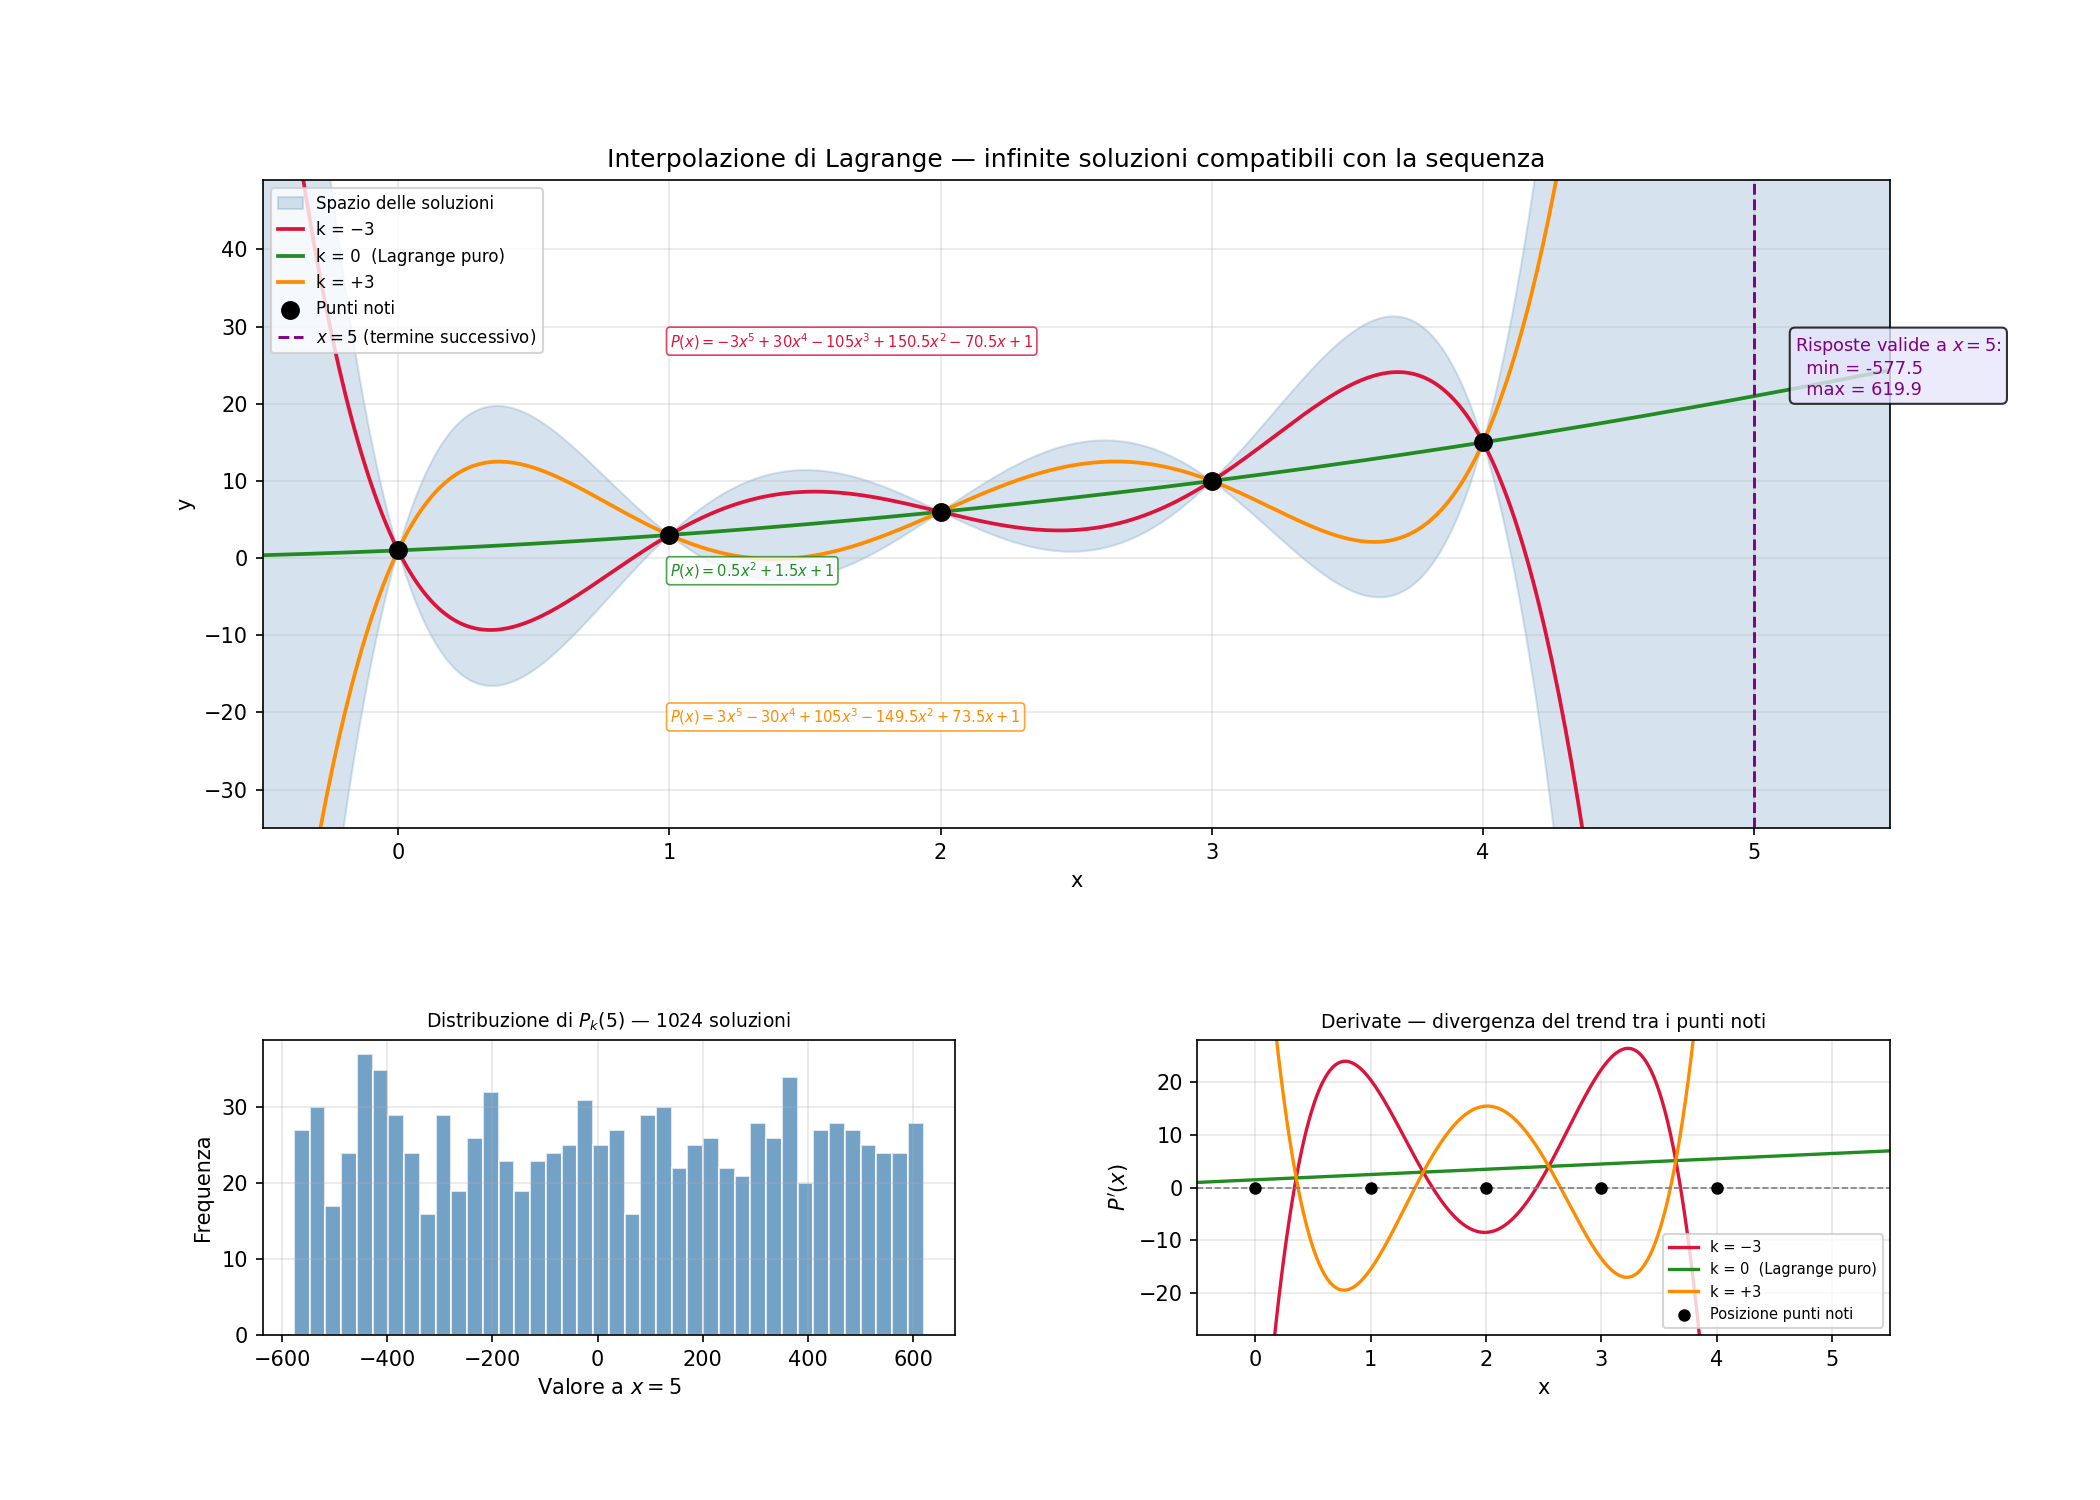
\includegraphics[width=\linewidth]{lagrange_plot.png}
    \caption{Visualizzazione della famiglia di interpolanti $P_k(x)=P(x)+kW(x)$
    prodotta dal codice del repository. L'area azzurra mostra l'inviluppo delle
    soluzioni campionate; le tre curve colorate mostrano alcuni esempi singoli;
    l'istogramma illustra la distribuzione dei valori ottenibili nel punto
    successivo; il pannello delle derivate evidenzia quanto possano divergere i
    comportamenti tra i punti osservati pur coincidendo esattamente su di essi.}
    \label{fig:plot}
\end{figure}

Il messaggio visivo della figura è semplice:
\begin{itemize}
    \item tutte le curve passano per gli stessi punti noti;
    \item tra un punto noto e l'altro, e soprattutto oltre l'ultimo punto,
          possono però separarsi anche molto;
    \item il valore nel punto successivo non è fissato dai dati, ma dipende dal
          parametro aggiuntivo $k$.
\end{itemize}

L'istogramma del valore a $x=n$ è quasi uniforme perché, fissati i dati, il
valore
\[
P_k(n)=P(n)+kW(n)
\]
dipende linearmente da $k$. Campionare uniformemente $k$ significa quindi
campionare uniformemente anche il valore previsto nel punto successivo, salvo
gli effetti numerici del campionamento finito.

\section{Che cos'è il fattore \texorpdfstring{$g$}{g}}
\label{sec:g}

\subsection{Origine storica dell'idea}

Il fattore $g$ prende il nome dalla parola inglese \emph{general}. La nozione
risale a Spearman, che osservò un fatto empirico robusto: punteggi ottenuti da
persone diverse in prove cognitive differenti tendono a essere positivamente
correlati tra loro~\cite{spearman1904}. In forma intuitiva:

\begin{quote}
chi va relativamente bene in una prova di ragionamento verbale tende, in media,
ad andare relativamente bene anche in prove numeriche, spaziali o di memoria,
pur con ovvie eccezioni e differenze di profilo.
\end{quote}

Questa regolarità viene spesso chiamata \emph{positive manifold}, cioè
\emph{manifold positivo delle correlazioni}. È uno dei risultati più replicati
nella psicometria dell'intelligenza~\cite{kovacs2016, vandermaas2006}.

\subsection{Definizione intuitiva}

Il fattore $g$ non è una domanda, non è un singolo compito e non è nemmeno un
numero letto direttamente da un termometro psicologico. È un \emph{fattore
latente}: una variabile non osservata direttamente, introdotta per spiegare la
porzione di varianza che più prove cognitive sembrano condividere.

Detto in modo ancora più semplice:
\begin{quote}
$g$ è il nome dato alla parte comune che emerge quando molte prove cognitive
diverse ``si muovono insieme'' nei dati.
\end{quote}

Questo punto è essenziale. Il fattore $g$ è una costruzione statistica
interpretata teoricamente, non un oggetto immediatamente osservabile.

\subsection{Che cosa \emph{non} è g}

Per evitare equivoci, conviene elencare alcune distinzioni.

\begin{itemize}
    \item \textbf{$g$ non coincide con il QI grezzo.} Un punteggio di QI è in
          genere un indice standardizzato ricavato da una batteria specifica;
          $g$ è il fattore latente comune stimato a partire dalle relazioni tra
          prove.
    \item \textbf{$g$ non esaurisce ogni teoria dell'intelligenza.} Esistono
          modelli gerarchici, modelli a fattori multipli e interpretazioni
          alternative del manifold positivo~\cite{cattell1963, carroll1993,
          sternberg1985, sternberg1999, kovacs2016, vandermaas2006}.
    \item \textbf{$g$ non implica automaticamente una causa unica semplice.}
          Alcuni autori lo interpretano come indice di una capacità generale;
          altri come risultato emergente dell'interazione tra processi cognitivi
          parzialmente sovrapposti~\cite{kovacs2016, vandermaas2006}.
\end{itemize}

\subsection{Il rapporto tra g, abilità ampie e abilità specifiche}

La letteratura psicometrica contemporanea descrive spesso l'intelligenza in modo
gerarchico. In modelli ispirati ai lavori di Cattell, Horn e Carroll, si
distinguono almeno tre livelli concettuali~\cite{cattell1963, carroll1993}:
\begin{enumerate}[label=\arabic*.]
    \item \textbf{abilità specifiche}:
          prestazioni in compiti circoscritti;
    \item \textbf{abilità ampie}:
          per esempio intelligenza fluida ($G_f$), intelligenza cristallizzata
          ($G_c$), memoria, velocità di elaborazione;
    \item \textbf{fattore generale}:
          la componente comune che sovrasta più abilità ampie.
\end{enumerate}

In questo linguaggio, gli item di sequenza vengono in genere interpretati come
prove che caricano soprattutto su capacità di ragionamento astratto e di
induzione di regole, spesso vicine a ciò che viene chiamato intelligenza
fluida. Ma il fatto che un item carichi su $g$ non significa che il suo
contenuto semantico sia irrilevante. È proprio qui che nasce il problema della
validità di costrutto.

\section{Come si calcola il fattore \texorpdfstring{$g$}{g}}
\label{sec:gcalc}

\subsection{Idea generale}

Dire che ``si calcola $g$'' può trarre in inganno. In realtà, non si misura
$g$ come si misura la temperatura con un termometro. Più precisamente:
\begin{enumerate}[label=\arabic*.]
    \item si raccolgono i punteggi di molte persone in molte prove cognitive;
    \item si osserva come questi punteggi correlano tra loro;
    \item si stima un modello statistico che riassume la parte condivisa delle
          prestazioni.
\end{enumerate}

Il risultato finale è una stima di un fattore latente comune. Questa stima
dipende sempre, almeno in parte, dalla batteria scelta, dal campione esaminato
e dal metodo statistico usato.

\subsection{Le fasi del calcolo, spiegate senza gergo inutile}

\begin{table*}[t]
    \centering
    \begin{tabular}{>{\raggedright\arraybackslash}p{1.8cm} >{\raggedright\arraybackslash}p{4.2cm} >{\raggedright\arraybackslash}p{7.2cm}}
        \toprule
        \textbf{Fase} & \textbf{Operazione} & \textbf{Significato intuitivo} \\
        \midrule
        1 & Somministrare una batteria di prove diverse & Serve osservare prestazioni su compiti non identici, per capire che cosa abbiano in comune. \\
        2 & Standardizzare i punteggi & I test usano scale diverse; la standardizzazione li rende confrontabili. \\
        3 & Costruire la matrice di correlazione & Si misura quanto i risultati nelle varie prove tendano a salire e scendere insieme. \\
        4 & Estrarre il fattore comune dominante & Si stima la componente latente che spiega la quota più ampia della covariazione condivisa. \\
        5 & Stimare i \emph{loadings} & Per ogni prova si valuta quanto essa dipenda dal fattore generale. \\
        6 & Calcolare i \emph{factor scores} individuali & Per ogni persona si produce una stima della sua posizione sul fattore generale, data quella batteria e quel metodo. \\
        \bottomrule
    \end{tabular}
    \caption{Schema intuitivo della stima del fattore $g$.}
    \label{tab:gsteps}
\end{table*}

\subsection{Passo 1: raccolta dei punteggi}

Supponiamo di avere $N$ persone e $p$ prove cognitive. Indichiamo con
$x_{ij}$ il punteggio della persona $i$ nella prova $j$. I dati grezzi
formano quindi una matrice $N \times p$.

Esempio intuitivo: ogni riga è una persona, ogni colonna è una prova
(vocabolario, analogie, serie numeriche, rotazioni mentali, memoria, e così
via).

\subsection{Passo 2: standardizzazione}

Le prove possono avere scale molto diverse. Una prova può andare da $0$ a $20$,
un'altra da $200$ a $800$. Per renderle confrontabili si trasformano spesso in
punteggi standardizzati:
\begin{equation}
z_{ij}=\frac{x_{ij}-\bar{x}_j}{s_j},
\label{eq:zscore}
\end{equation}
dove $\bar{x}_j$ è la media della prova $j$ e $s_j$ la sua deviazione
standard.

Interpretazione: $z_{ij}=0$ significa ``nella media''; $z_{ij}=1$ significa
``una deviazione standard sopra la media''; $z_{ij}=-1$ significa ``una
deviazione standard sotto la media''.

\subsection{Passo 3: matrice di correlazione}

Una volta standardizzati i punteggi, si calcola la matrice di correlazione
\[
R=(r_{jk})_{j,k=1}^{p},
\]
dove ciascun coefficiente $r_{jk}$ misura il grado di associazione tra le prove
$j$ e $k$.

Se molti coefficienti sono positivi, si osserva il manifold positivo che ha
motivato storicamente l'introduzione di $g$~\cite{spearman1904}.

\subsection{Passo 4: modello fattoriale}

In una versione semplificata a un solo fattore, il punteggio standardizzato
della persona $i$ nella prova $j$ viene scritto come
\begin{equation}
z_{ij}=\lambda_j g_i + \epsilon_{ij}.
\label{eq:factor}
\end{equation}

Qui:
\begin{itemize}
    \item $g_i$ è la posizione latente della persona $i$ sul fattore generale;
    \item $\lambda_j$ è il \emph{loading} della prova $j$ su $g$;
    \item $\epsilon_{ij}$ raccoglie ciò che resta: componente specifica della
          prova, errore di misura, variabilità non spiegata dal fattore comune.
\end{itemize}

Se $\lambda_j$ è grande in valore assoluto, quella prova dipende molto dal
fattore generale. Se è piccolo, la prova riflette meno $g$ e più componenti
specifiche.

In termini matriciali, il modello di fattore comune può essere riassunto come
\begin{equation}
R \approx \Lambda\Lambda^\top + \Psi,
\label{eq:commonfactor}
\end{equation}
dove $\Lambda$ contiene i loadings e $\Psi$ la parte non condivisa.

\subsection{Passo 5: estrazione del fattore}

Dal punto di vista operativo, bisogna stimare i parametri del modello.
Esistono più procedure:
\begin{itemize}
    \item analisi fattoriale esplorativa;
    \item modelli fattoriali confermativi;
    \item modelli gerarchici o bifattoriali.
\end{itemize}

Tutti questi approcci cercano, in modi diversi, di riassumere la covariazione
tra prove. Il punto importante per il lettore non specialista è questo:

\begin{quote}
il valore di $g$ non cade fuori automaticamente dai dati; emerge da un modello
statistico scelto dal ricercatore.
\end{quote}

\subsection{Passo 6: calcolo del punteggio fattoriale individuale}

Una volta stimati i loadings, si può assegnare a ciascuna persona una stima del
suo punteggio su $g$, spesso indicata con $\hat{g}_i$. In forma schematica:
\begin{equation}
\hat{g}_i = w_1 z_{i1} + w_2 z_{i2} + \cdots + w_p z_{ip},
\label{eq:factorscore}
\end{equation}
dove i pesi $w_1,\ldots,w_p$ dipendono dal metodo di scoring adottato
(regression scoring, Bartlett scoring, ecc.).

Questo aspetto è spesso trascurato nelle discussioni divulgative:
\begin{quote}
un punteggio individuale di $g$ è una \emph{stima modellistica}, non una misura
osservata direttamente.
\end{quote}

\subsection{Un mini-esempio puramente illustrativo}

Supponiamo che una batteria contenga quattro prove: vocabolario, serie
numeriche, rotazione mentale e memoria di lavoro. Dopo l'analisi fattoriale, si
ottengono loadings ipotetici come quelli della Tabella~\ref{tab:loadings}.

\begin{table*}[t]
    \centering
    \begin{tabular}{lcc}
        \toprule
        \textbf{Prova} & \textbf{Loading su $g$} & \textbf{Varianza comune stimata ($\lambda^2$)} \\
        \midrule
        Vocabolario & 0.72 & 0.52 \\
        Serie numeriche & 0.78 & 0.61 \\
        Rotazione mentale & 0.69 & 0.48 \\
        Memoria di lavoro & 0.64 & 0.41 \\
        \bottomrule
    \end{tabular}
    \caption{Esempio illustrativo di loadings fattoriali. I valori sono
    mostrati solo a scopo didattico.}
    \label{tab:loadings}
\end{table*}

Una persona che ottenga punteggi standardizzati alti in più prove riceverà, di
norma, una stima di $\hat{g}$ più alta. Ma questa stima dipende dai pesi, dai
loadings e dalla batteria. Cambiando test o metodo, si può ottenere una stima
non identica.

\subsection{Distinzione importante: primo componente principale e fattore g}

\begin{remark}
Nella pratica si sente talvolta dire che $g$ coincide con il primo componente
principale. La frase è comoda ma imprecisa. La PCA riassume la varianza totale
dei punteggi osservati; l'analisi fattoriale comune cerca invece di modellare la
varianza condivisa tra prove. I due risultati possono assomigliarsi, ma non sono
concettualmente la stessa cosa.
\end{remark}

\section{Che cosa segue per la validità di costrutto}
\label{sec:validity}

\subsection{Prima chiarificazione: la critica non dice che i test ``non misurano nulla''}

Questa è una distinzione decisiva. Dal fatto che un item di sequenza sia
sottodeterminato \emph{non} segue che ogni test di intelligenza sia inutile o
privo di potere predittivo. In effetti, l'esistenza del manifold positivo e la
capacità di alcune batterie di predire esiti educativi sono risultati ben
documentati~\cite{deary2007, jensen1998}.

La critica qui proposta è più circoscritta:
\begin{quote}
anche quando un test è utile, resta aperta la domanda se misuri esattamente il
costrutto che dichiara di misurare e se ogni suo item sia interpretabile nel
modo in cui viene normalmente presentato.
\end{quote}

\subsection{Che cos'è la validità di costrutto}

\begin{definition}[Validità di costrutto]
Un test possiede validità di costrutto se l'interpretazione dei suoi punteggi
come misure di un certo costrutto teorico è giustificata da evidenze e da una
teoria coerente del processo che genera le risposte~\cite{cronbach1955,
borsboom2004}.
\end{definition}

In forma intuitiva, la validità di costrutto risponde alla domanda:
\begin{quote}
``quando osservo questo punteggio, ho davvero buone ragioni per dire che sto
misurando proprio la proprietà psicologica dichiarata dal test?''
\end{quote}

Una buona correlazione con altri test o con alcuni esiti esterni è importante,
ma non esaurisce da sola il problema del significato del punteggio.

\subsection{Dove colpisce l'argomento della sottodeterminazione}

Nel caso degli item di completamento numerico, il punto non è che essi siano
sempre cattivi item. Il punto è che la loro interpretazione richiede una
precisazione in più.

Se la sequenza osservata non determina da sola una continuazione unica, allora
un punteggio pieno assegnato a una risposta specifica premia almeno una delle
seguenti capacità:
\begin{enumerate}[label=\arabic*.]
    \item riconoscere il pattern che il progettista del test \emph{intendeva};
    \item applicare un criterio implicito di semplicità o familiarità;
    \item accettare il framing della domanda, cioè l'idea che debba esistere una
          sola continuazione attesa;
    \item lavorare rapidamente entro convenzioni condivise e non esplicitate.
\end{enumerate}

Tutte queste abilità possono essere reali e utili. Ma non coincidono
automaticamente con ``intelligenza generale'' nel senso più ampio e filosofico
del termine.

\subsection{Il ruolo del fattore g nella difesa standard}

La difesa psicometrica standard procede spesso così:
\begin{enumerate}[label=\arabic*.]
    \item i punteggi a molti item cognitivi correlano positivamente;
    \item da questa struttura si estrae un fattore generale $g$;
    \item un item che carica su $g$ viene considerato un buon indicatore di
          intelligenza generale.
\end{enumerate}

Questo ragionamento non è privo di forza. Ma non chiude la questione. Un item
può caricare su $g$ e, al tempo stesso, richiedere competenze più specifiche di
quanto il nome ``intelligenza'' lasci intendere.

\subsection{La circolarità da evitare}

Qui serve molta precisione. Sarebbe scorretto dire che tutta la psicometria di
$g$ è una tautologia vuota. Non lo è. Esistono dati reali, correlazioni
replicate e relazioni con esiti esterni. Tuttavia esiste una \emph{circolarità
parziale} che merita attenzione:

\begin{itemize}
    \item gli item vengono selezionati anche perché mostrano buone correlazioni
          con altre prove della batteria;
    \item il fattore $g$ viene stimato a partire da batterie costruite in questo
          modo;
    \item il fatto che un item carichi su $g$ dice molto sulla sua coerenza con
          la batteria, ma da solo non risponde interamente alla domanda sul
          contenuto cognitivo che l'item premia.
\end{itemize}

In altre parole, \emph{loading alto su $g$} e \emph{trasparenza del costrutto}
non sono sinonimi.

\subsection{Che cosa misura plausibilmente un item di sequenza}

Alla luce di tutto quanto precede, una formulazione più prudente e più precisa
potrebbe essere questa:

\begin{quote}
gli item di sequenza misurano, almeno in parte, la capacità di inferire una
regola convenzionale ritenuta appropriata dal contesto del test, sotto vincoli
di tempo e con informazione incompleta.
\end{quote}

Questa formulazione è meno enfatica di ``misura l'intelligenza in generale'',
ma probabilmente più vicina a ciò che il comportamento osservato supporta
davvero.

\section{Confronto con prospettive più ampie sull'intelligenza}
\label{sec:broader}

Le critiche alla riduzione dell'intelligenza a un singolo indice non sono nuove.
Sternberg ha sostenuto, in forme diverse, che le prove tradizionali catturano
solo una parte delle abilità rilevanti e che occorre tenere conto anche di
componenti creative, pratiche e meta-cognitive~\cite{sternberg1985,
sternberg1999}. Stanovich ha insistito sul fatto che i test di intelligenza,
pur utili, lasciano fuori tratti cognitivi centrali per il giudizio razionale,
la valutazione delle prove e il buon ragionamento quotidiano~\cite{stanovich2009}.

Questa letteratura non prova da sola la nostra tesi matematica, ma la colloca in
un quadro più ampio: un test può essere empiricamente utile e tuttavia
incompleto rispetto a ciò che molte persone intendono, nel linguaggio ordinario,
con la parola ``intelligenza''.

Gli item di sequenza sono un caso particolarmente istruttivo proprio perché
mostrano, in forma molto concentrata, la distanza tra:
\begin{itemize}
    \item una prestazione ben definita all'interno di una convenzione;
    \item la pretesa più ambiziosa di misurare una capacità generale di
          ragionamento.
\end{itemize}

\section{Limiti dell'argomento}
\label{sec:limits}

Un paper rigoroso deve indicare non solo ciò che mostra, ma anche ciò che non
mostra. I limiti principali sono quattro.

\begin{enumerate}[label=\arabic*.]
    \item \textbf{Non tutti gli item di test sono ugualmente ambigui.}
          Alcuni problemi includono indizi contestuali o vincoli impliciti molto
          forti, che riducono lo spazio delle interpretazioni ragionevoli.

    \item \textbf{La sottodeterminazione matematica non annulla l'utilità
          operativa.} In molti contesti pratici può essere perfettamente utile
          verificare se una persona riconosca rapidamente pattern semplici e
          convenzionali.

    \item \textbf{Un singolo item non coincide con l'intera batteria.}
          Le batterie psicometriche aggregano molte prove proprio per ridurre
          l'errore casuale e aumentare l'affidabilità complessiva.

    \item \textbf{L'argomento colpisce soprattutto l'interpretazione del
          costrutto.} Il bersaglio principale non è la mera esistenza di
          correlazioni o di validità predittiva, ma il salto concettuale che
          porta da tali correlazioni all'affermazione che una certa risposta
          numerica sia l'unica logicamente corretta e che il suo riconoscimento
          coincida senz'altro con l'intelligenza generale.
\end{enumerate}

\section{Conclusioni}
\label{sec:conclusion}

La tesi centrale dell'articolo può essere riassunta in una frase:
\begin{quote}
una sequenza finita, presa da sola, non determina in modo univoco il termine
successivo; per ottenere una risposta unica bisogna introdurre vincoli o
convenzioni ulteriori.
\end{quote}

Il teorema di interpolazione di Lagrange e la costruzione della famiglia
$P(x)+W(x)H(x)$ permettono di dimostrare questo punto in modo semplice, formale
e generalissimo. Da qui non segue che i test di intelligenza siano privi di
valore, ma segue che l'interpretazione dei loro item di sequenza deve essere più
sobria e più precisa.

Il fattore $g$, spiegato correttamente, è un fattore latente estratto dalla
struttura di correlazione tra prove cognitive. È uno strumento statistico
potente e storicamente centrale nella psicometria. Ma il fatto che un item
carichi su $g$ non basta, da solo, a risolvere ogni questione relativa al
significato dell'item. La validità di costrutto richiede anche un'analisi del
processo cognitivo che l'item premia.

Nel caso degli item di completamento numerico, la conclusione più difendibile è
quindi la seguente: essi misurano certamente qualcosa, ma quel qualcosa è meglio
descritto come capacità di inferire e applicare una regola convenzionale attesa
in un contesto di test, piuttosto che come accesso immediato e non problematico
all'intelligenza in senso generale.

Una progettazione più trasparente potrebbe migliorare questo quadro in almeno due
modi:
\begin{enumerate}[label=\arabic*.]
    \item esplicitando la classe di regole ammissibili;
    \item premiando non solo la risposta finale, ma anche la qualità della
          giustificazione e la capacità di riconoscere quando il problema è
          sottovincolato.
\end{enumerate}

\appendix

\section{Glossario essenziale}
\label{sec:glossary}

\begin{description}[style=nextline, leftmargin=2.7cm]
    \item[Interpolazione]
    Costruzione di una funzione che passi esattamente per un insieme di punti
    dati.

    \item[Sottodeterminazione]
    Situazione in cui i dati disponibili non bastano a selezionare una soluzione
    unica senza ipotesi aggiuntive.

    \item[Parsimonia]
    Preferenza per spiegazioni o modelli più semplici, a parità di compatibilità
    con i dati.

    \item[Correlazione]
    Misura di quanto due variabili tendano a crescere o diminuire insieme.

    \item[Variabile latente]
    Variabile teorica non osservata direttamente, introdotta per spiegare
    regolarità nei dati osservati.

    \item[Loading fattoriale]
    Coefficiente che indica quanto una prova sia associata a un fattore latente.

    \item[Factor score]
    Stima numerica, per un individuo, della sua posizione su un fattore latente.

    \item[Validità di costrutto]
    Giustificazione teorica ed empirica dell'interpretazione di un punteggio come
    misura di una certa proprietà psicologica.
\end{description}

\section*{Appendice tecnica sul repository}
\addcontentsline{toc}{section}{Appendice tecnica sul repository}

Il repository allegato contiene una dimostrazione computazionale coerente con la
tesi matematica del testo:
\begin{itemize}
    \item \texttt{lagrange.cu} calcola in parallelo la famiglia di polinomi
          perturbati;
    \item \texttt{output.csv} contiene l'inviluppo numerico delle soluzioni;
    \item \texttt{plot.py} costruisce la figura finale;
    \item \texttt{lagrange\_plot.png} visualizza il risultato.
\end{itemize}

Questa parte empirica non sostituisce il ragionamento teorico, ma ha un valore
pedagogico importante: rende visibile, in un colpo d'occhio, quanto ampia possa
essere la famiglia di soluzioni compatibili con gli stessi punti osservati.

\begin{thebibliography}{99}

\bibitem{spearman1904}
Spearman, C. (1904).
``General Intelligence,'' Objectively Determined and Measured.
\textit{The American Journal of Psychology}, 15(2), 201--293.
doi:10.2307/1412107

\bibitem{cronbach1955}
Cronbach, L.~J., \& Meehl, P.~E. (1955).
Construct validity in psychological tests.
\textit{Psychological Bulletin}, 52(4), 281--302.
doi:10.1037/h0040957

\bibitem{cattell1963}
Cattell, R.~B. (1963).
Theory of fluid and crystallized intelligence: A critical experiment.
\textit{Journal of Educational Psychology}, 54(1), 1--22.
doi:10.1037/h0046743

\bibitem{carroll1993}
Carroll, J.~B. (1993).
\textit{Human Cognitive Abilities: A Survey of Factor-Analytic Studies}.
Cambridge University Press.
doi:10.1017/CBO9780511571312

\bibitem{jensen1998}
Jensen, A.~R. (1998).
\textit{The g Factor: The Science of Mental Ability}.
Greenwood Publishing.

\bibitem{sternberg1985}
Sternberg, R.~J. (1985).
\textit{Beyond IQ: A Triarchic Theory of Human Intelligence}.
Cambridge University Press.

\bibitem{sternberg1999}
Sternberg, R.~J. (1999).
The theory of successful intelligence.
\textit{Review of General Psychology}, 3(4), 292--316.
doi:10.1037/1089-2680.3.4.292

\bibitem{borsboom2004}
Borsboom, D., Mellenbergh, G.~J., \& van Heerden, J. (2004).
The concept of validity.
\textit{Psychological Review}, 111(4), 1061--1071.
doi:10.1037/0033-295X.111.4.1061

\bibitem{vandermaas2006}
van der Maas, H.~L.~J., Dolan, C.~V., Grasman, R.~P.~P.~P., Wicherts, J.~M.,
Huizenga, H.~M., \& Raijmakers, M.~E.~J. (2006).
A dynamical model of general intelligence: The positive manifold of intelligence
by mutualism.
\textit{Psychological Review}, 113(4), 842--861.
doi:10.1037/0033-295X.113.4.842

\bibitem{deary2007}
Deary, I.~J., Strand, S., Smith, P., \& Fernandes, C. (2007).
Intelligence and educational achievement.
\textit{Intelligence}, 35(1), 13--21.
doi:10.1016/j.intell.2006.02.001

\bibitem{stanovich2009}
Stanovich, K.~E. (2009).
\textit{What Intelligence Tests Miss: The Psychology of Rational Thought}.
Yale University Press.

\bibitem{kovacs2016}
Kovacs, K., \& Conway, A.~R.~A. (2016).
Process overlap theory: A unified account of the general factor of intelligence.
\textit{Psychological Inquiry}, 27(3), 151--177.
doi:10.1080/1047840X.2016.1153946

\bibitem{taleb2019}
Taleb, N.~N. (2019).
\textit{IQ is largely a pseudoscientific swindle}.
Medium. \url{https://medium.com/incerto/iq-is-largely-a-pseudoscientific-swindle-f131c101ba39}

\bibitem{gould1981}
Gould, S.~J. (1981).
\textit{The Mismeasure of Man}.
W.~W. Norton \& Company.

\bibitem{gardner1983}
Gardner, H. (1983).
\textit{Frames of Mind: The Theory of Multiple Intelligences}.
Basic Books.

\bibitem{knill2014}
Knill, O. (2014).
\textit{Math 1a — Sequences and IQ tests}.
Harvard University, course notes.

\end{thebibliography}

\end{document}
